To access the web application, navigate to a domain and directory that publicly serves the web page. An example of this could be: scratchy.cs.umu.se:8000/app/.
All functionality of the web application is (or rather should be) fairly self-explanatory and intuitive. A short description and explanation will be given for each component that have been implemented so far.
\subsection{Using the interface}
This section will describe how to use the interface and how to interact with it.
\subsubsection{Start view}
%figure 1
\begin{figure}[h]
\centering
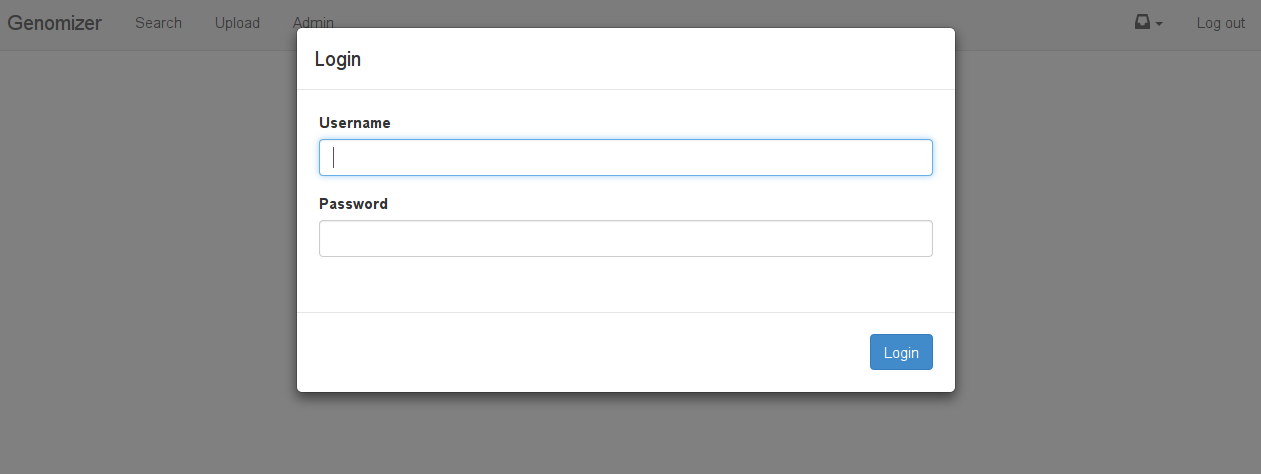
\includegraphics[width=1\textwidth]{web_search_login.png}
\caption{\label{fig:web_search_login} The login modal.}
\end{figure}
When first enetering the webpage the login modal in \refer{fig:web_search_login} is shown and the user will have to enter his username and password to gain access to the application.

%figure 2
\begin{figure}[h]
\centering
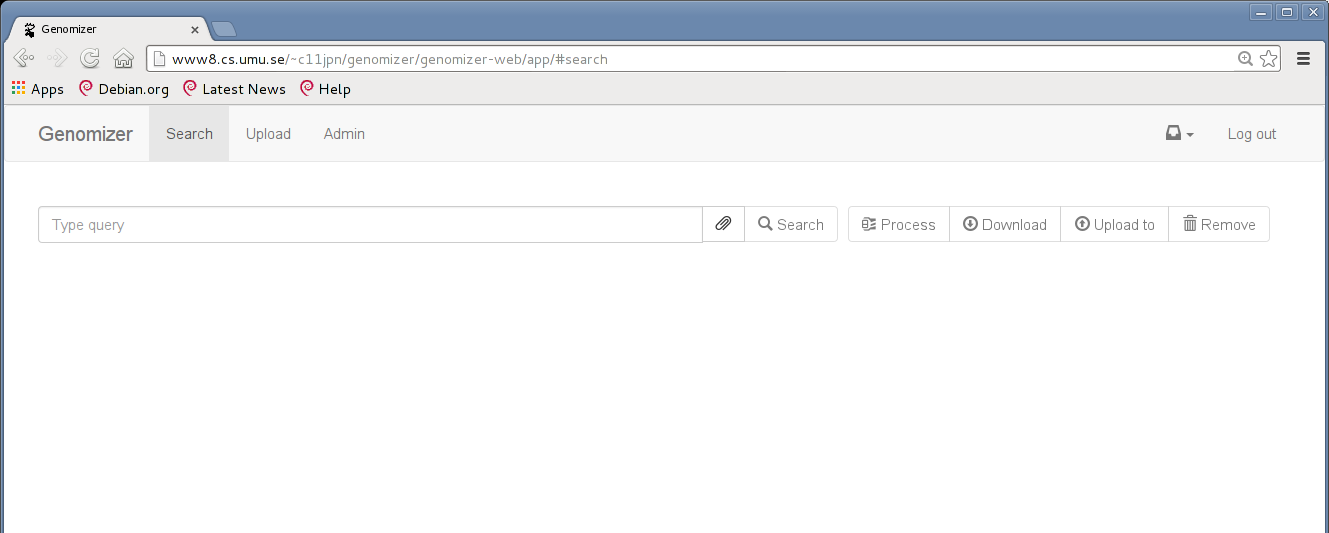
\includegraphics[width=1\textwidth]{web_search_welcome.png}
\caption{\label{fig:web_search_welcome} The welcome screen of the webpage.}
\end{figure}

When the user has logged in, the user is taken to the search page as shown in \refer{fig:web_search_welcome}.

The navigation bar at the top has four buttons to the left and two buttons to the right with the following functionality:
\begin{itemize}
	\item Clicking the “Genomizer” logo should take the user right back to the start view.
	\item The “Search” button will bring up the search view where the user can enter search strings to be sent to the server, and view search results.
	\item The “Upload” button will bring up the upload view where the user can select files to be uploaded and input annotation to a new experiment.
	\item The “Admin” button will be shown for administrators, that is where the administrator can handle users and annotations.
    \item The inbox icon on the left side opens a process status dropdown.
    \item The "Log out" button will log out the user.
\end{itemize}
This navigation bar is persistent through all subpages and can easily be accessed.

\subsubsection{Search view}

Below the navigation bar a “search-and-functionality” bar is visible, there is a search field and there are six buttons, Query-builder, Search, Download, Upload to and process. However, when first entering the page some buttons will be disabled. When you enter something in the search field the search button will become enabled and clickable. To search the user can either write a pubmed style query (for example: Exp1[ExpID]) or use the query builder, by clicking the paperclip icon.

%figure BILD
\begin{figure}[h]
\centering
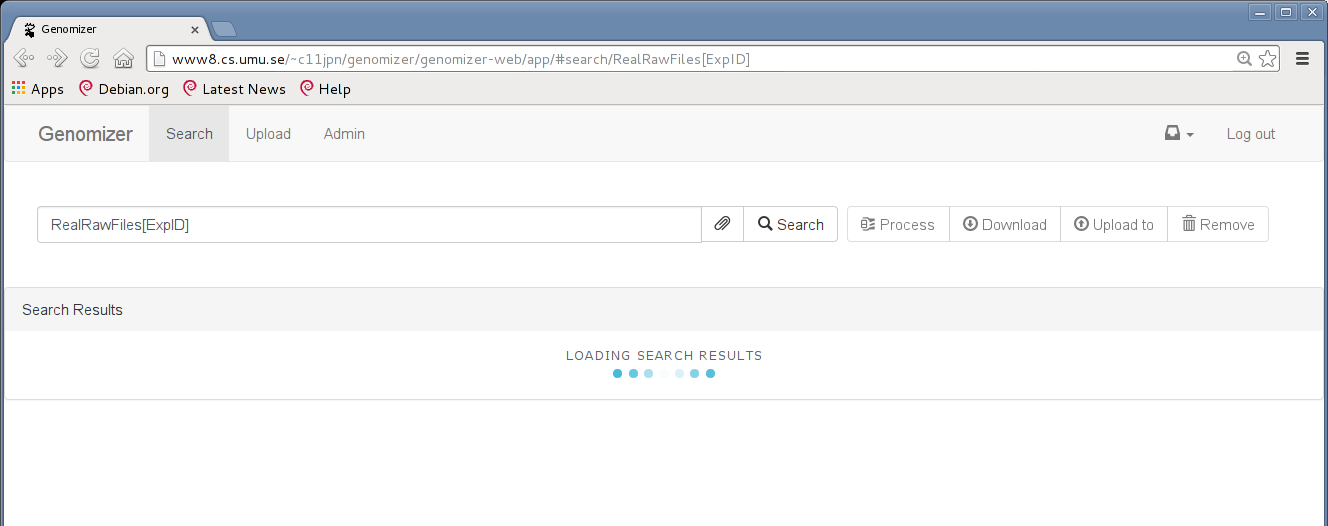
\includegraphics[width=1\textwidth]{web_search_searching.png}
\caption{\label{fig:web_search_searching}will be shown while searching for data in the database before any results are found.}
\end{figure}

After having typed a query and pressed search, the search results will load displaying the loading spinner as can be seen in figure \refer{fig:web_search_searching}.
%figure x3
\begin{figure}[h]
\centering
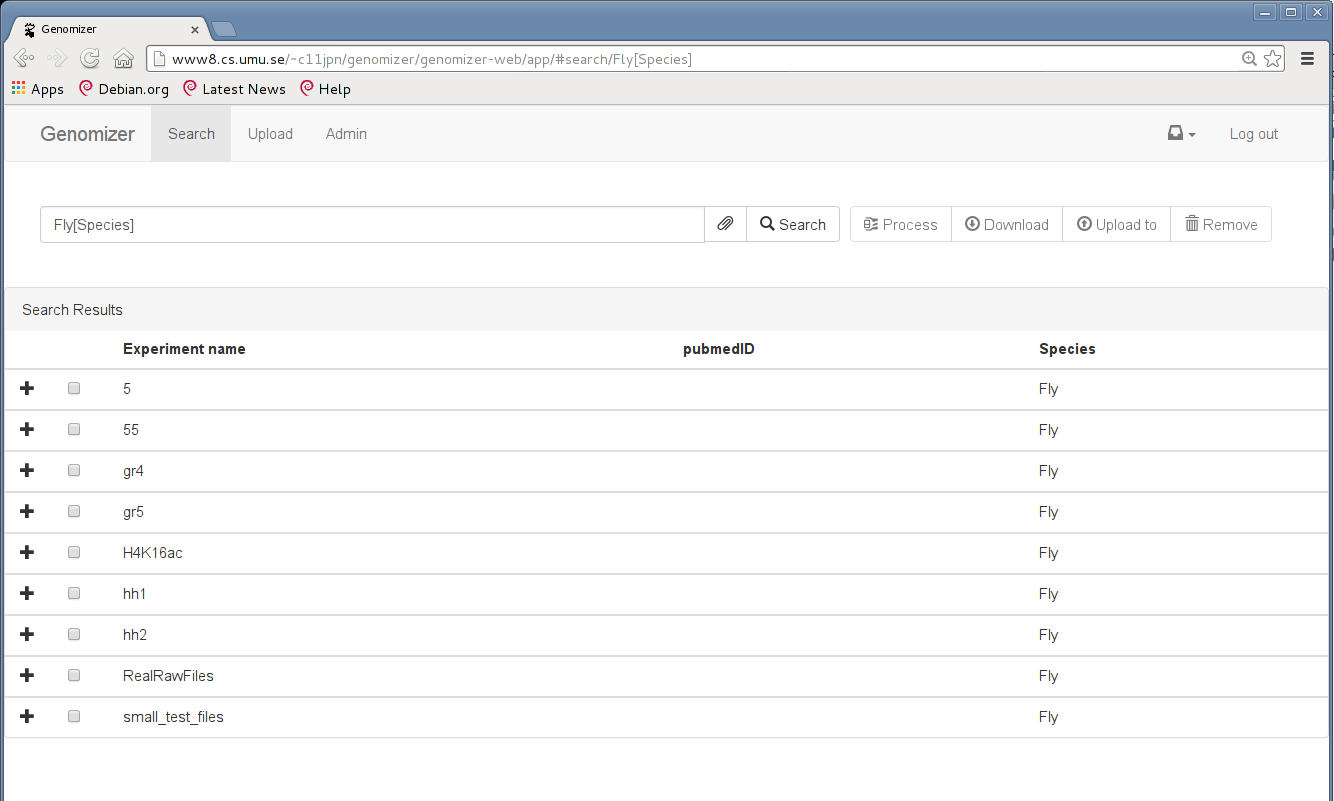
\includegraphics[width=1\textwidth]{web_search_searchTab.png}
\caption{\label{fig:web_search_searchTab}the search tab after a search for ‘Fly[Species]’.}
\end{figure}

The view shown in \refer{fig:web_search_searchTab} contains two major elements; a “search-and-functionality” bar and a list of search results retrieved after searching for ‘Exp1[ExpID]’. The buttons next to the search bar do the following: 
\begin{itemize}
	\item The paperclip brings up a Query builder.
	\item “Search” searches for the query in the search bar. 
	\item “Process” brings up a new window in front of the search view with options for file processing. This feature is demonstrated further in \refer{fig:web_process_modalView}.
    \item “Download” downloads the selected files. 
    \item "Upload to" opens the upload view with the selected experiments selected where the user can upload new files to a already existing experiment.
    \item "Remove" opens a new view where the files which are going to be deleted are represented and a confrimation dialog that the user really wants to delete those files and experiments.
\end{itemize}
\begin{figure}[h]
\centering
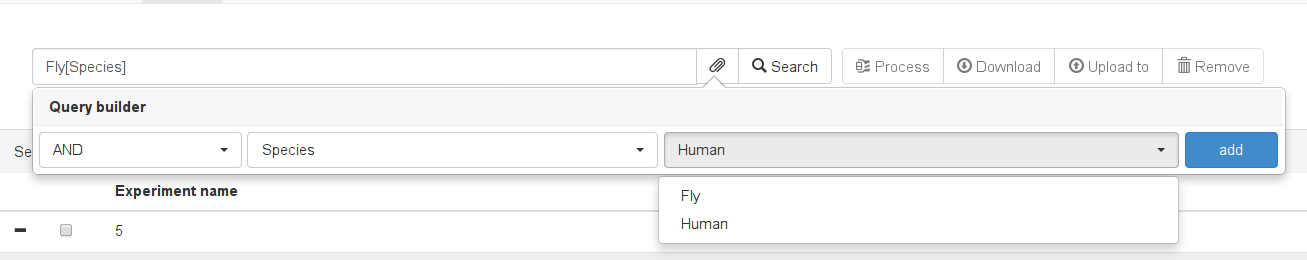
\includegraphics[width=1\textwidth]{web_search_queryBuilder.png}
\caption{\label{fig:web_search_queryBuilder}The query builder.}
\end{figure}
The search query builder as shown in \refer{fig:web_search_queryBuilder} can be used to easily build pubmed-styled search queries. Just select a value in the three fields and press add. The correct pubmed-styled query will be shown in the search field and the three query fields will be reset so the user can add more things to search for in their query.

Below the search bar in \refer{fig:web_search_searchTab} is the “search results” list. This list contains all experiments returned from a search. Every experiment can be expanded to show the file types it contains. Each file type can be expanded to show all files of that type in the experiment. All files and experiments has a check box next to it that is used to select what to process, download, remove or upload to.
%figure x4
\begin{figure}[h]
\centering
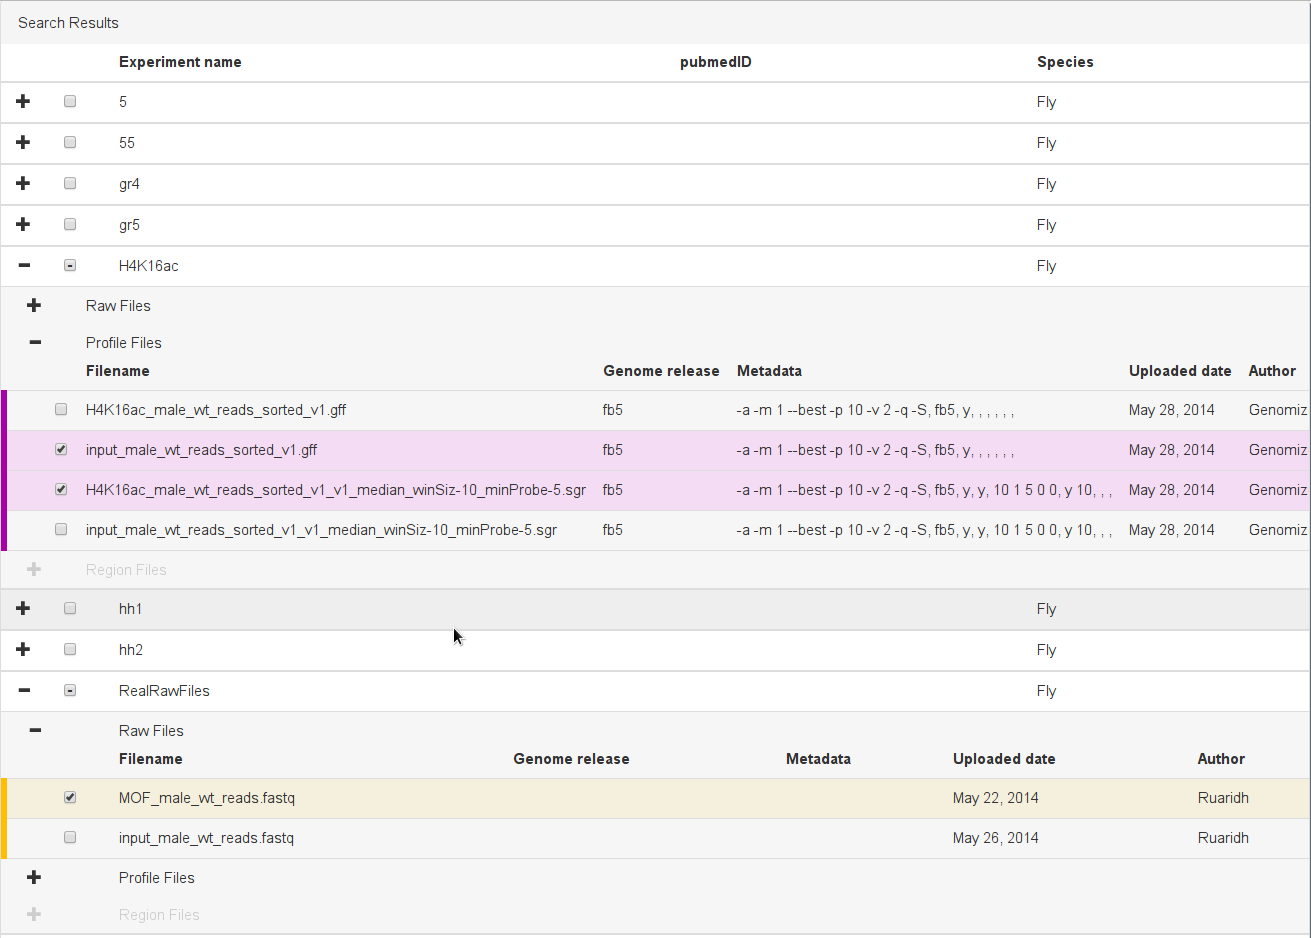
\includegraphics[width=1\textwidth]{web_search_searchResult.png}
\caption{\label{fig:web_search_searchResult}the search results table zoomed in, displaying a raw file’s information after having expanded an experiment.}
\end{figure}
\FloatBarrier
If a search is successful, you will be met with a table of results. This table has a header displaying the annotation types. Below that, all the experiments returned from a search and their corresponding annotation values, as can be seen in \refer{fig:web_search_searchResult}.
%figure BILD PÅ NO SEARCH RESULTS
\begin{figure}[h]
\centering
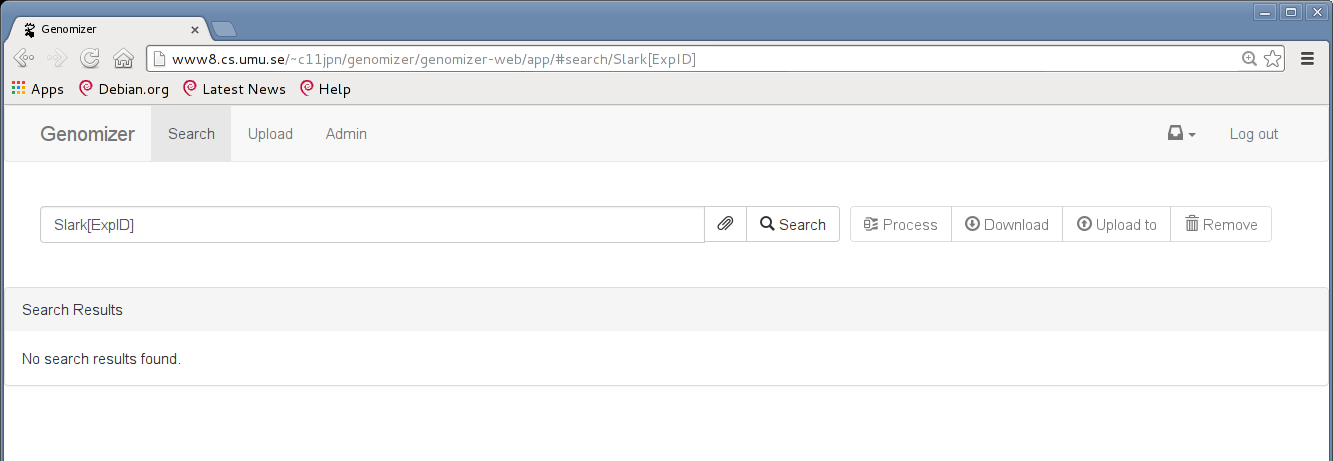
\includegraphics[width=1\textwidth]{web_search_noResult.png}
\caption{\label{fig:web_search_noResult}tells the user that no data was found given the search query entered by the user.}
\end{figure}
\FloatBarrier

If the search is unsuccessful, the Search Results table will be empty stating “No search results found” as can be seen in \refer{fig:web_search_noResult}.

\subsubsection{The processing modal}
%figure X6
\begin{figure}[h]
\centering
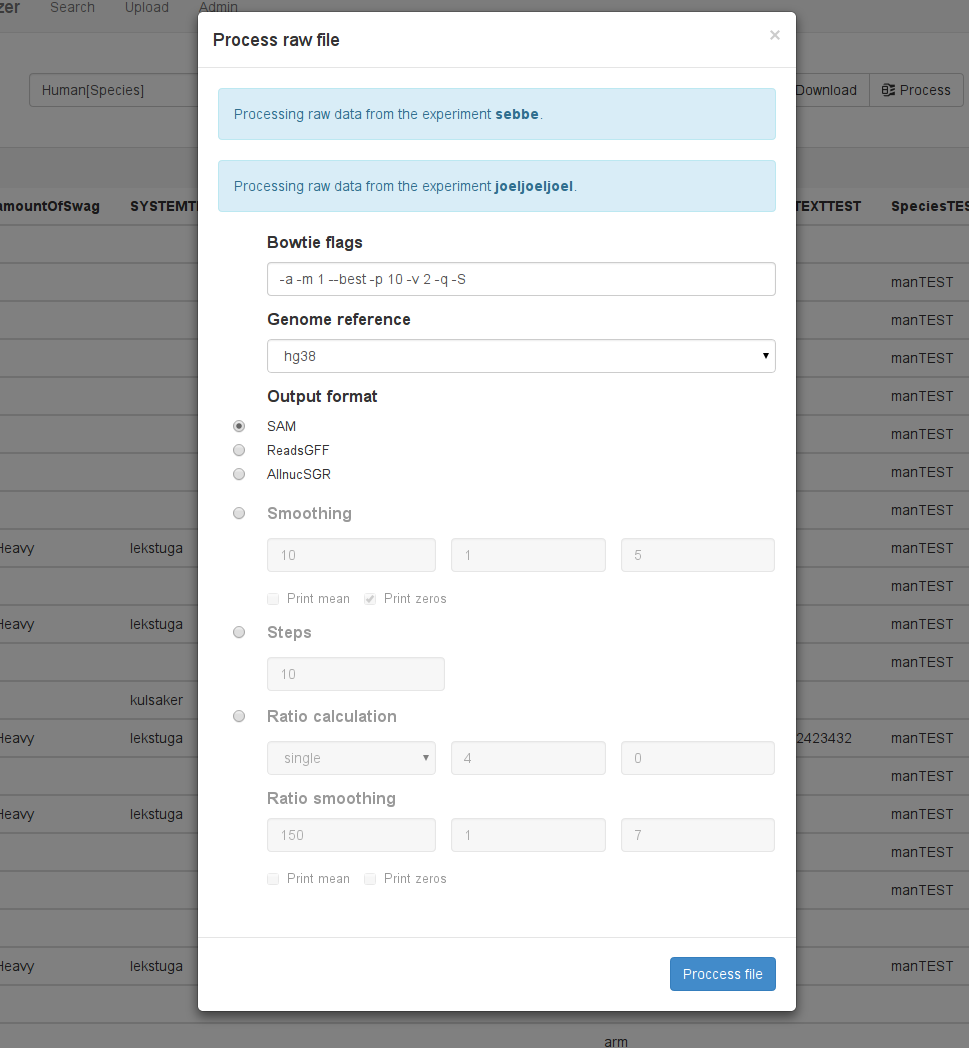
\includegraphics[width=1\textwidth]{web_process_modalView.png}
\caption{\label{fig:web_process_modalView}The process file modal.}
\end{figure}
\FloatBarrier
When the user has selected some files that are going to be processed the user will be presented with the view from \refer{fig:web_process_modalView}. The user can here choose which level of processing should be done on the raw files. By clicking the radio buttons on the left side that much processing will be done on the raw files. All the steps above the selected will also be executed since they are needed to reach that level of processing.
At the top of the modal the experiments currently going to processing are presented.
\begin{figure}[h]
\centering
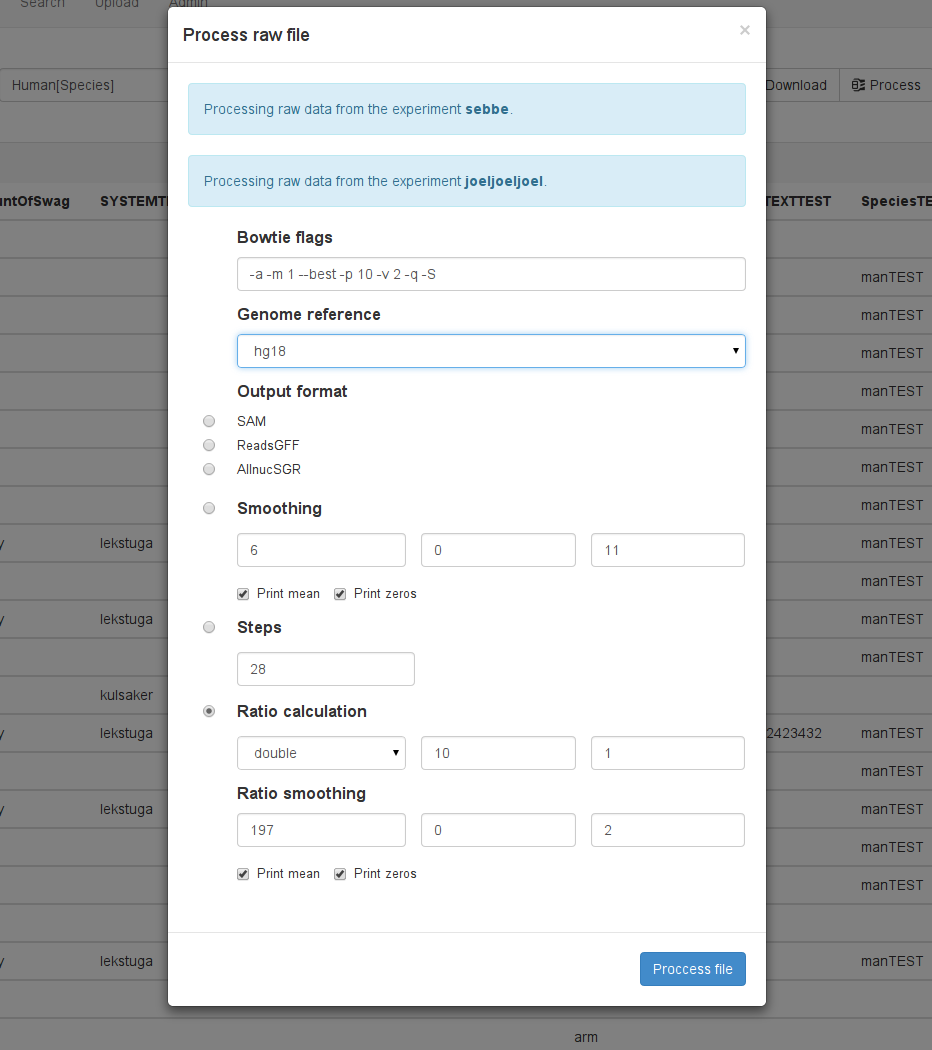
\includegraphics[width=1\textwidth]{web_process_modalValues.png}
\caption{\label{fig:web_process_modalValues}The process modal with selected parameters.}
\end{figure}
\FloatBarrier
When the user has decided the parameters as shown in \refer{fig:web_process_modalValues} and wants to start the processing the process button in the bottom right should be pressed. 
\begin{figure}[h]
\centering
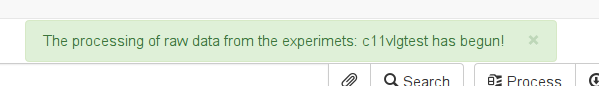
\includegraphics[width=1\textwidth]{web_process_success.png}
\caption{\label{fig:web_process_success}Success message.}
\end{figure}
\FloatBarrier
When results are recived from the server and they were all successfull the processing modal will dissapear and a success message indicating that the processing is starting will be displayed to the user like in \refer{fig:web_process_success}.
\begin{figure}[h]
\centering
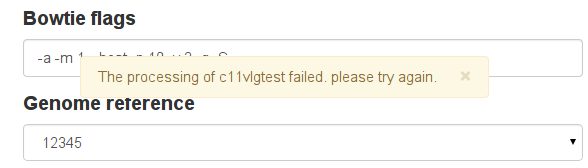
\includegraphics[width=1\textwidth]{web_process_notSuccess.png}
\caption{\label{fig:web_process_notSuccess}All did not success message.}
\end{figure}
If some of the files that was going to be processed did for some reason fail the user will learn this by a warning message that tells the user which experiment did not start processing and which did as shown in \refer{fig:web_process_notSuccess}. The ones which started to process will be removed from the modal and the ones that did not start to process will remain. The user can now choose other parameters or do something else to make it work and try to submit a processing request again
\pagebreak
\subsubsection{The remove modal}
\begin{figure}[h]
\centering
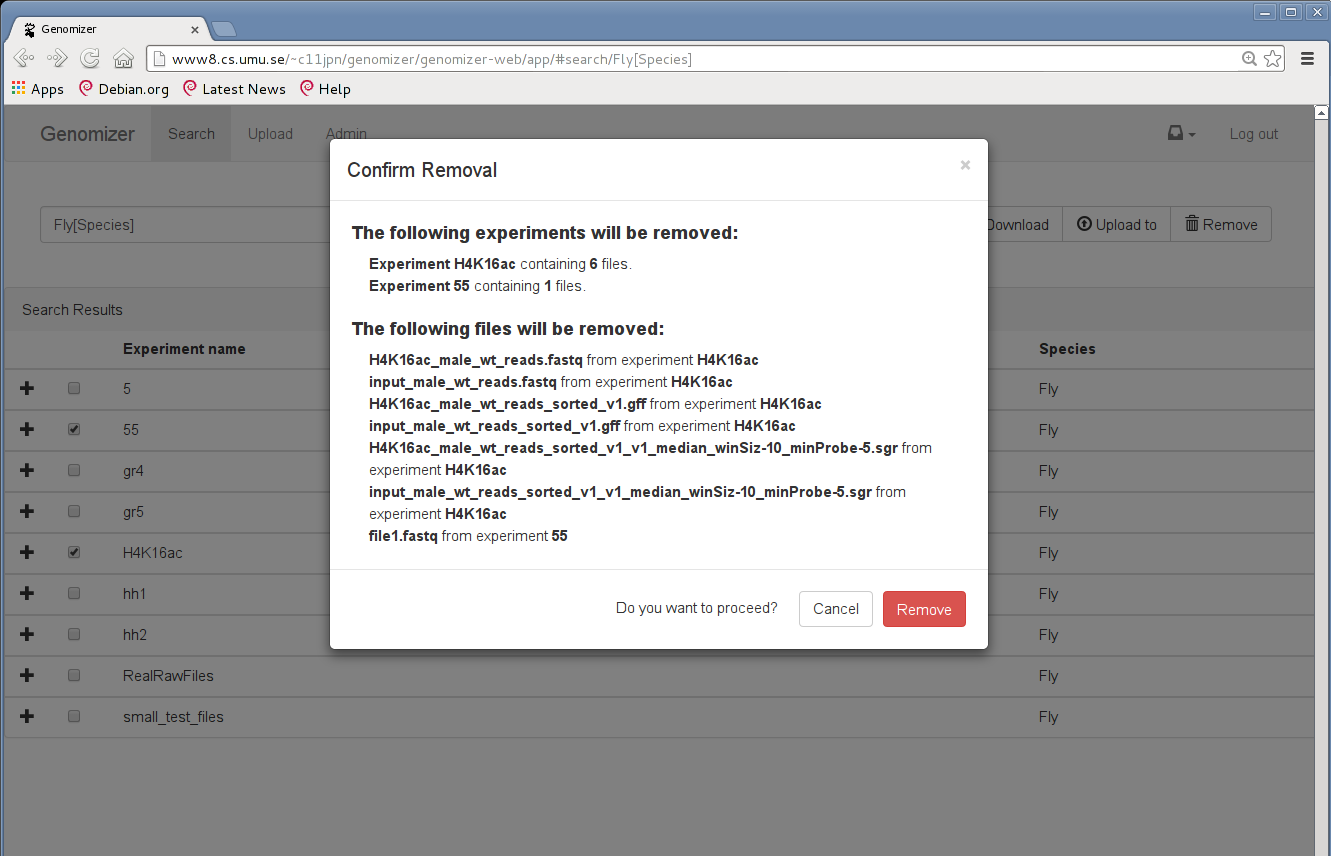
\includegraphics[width=0.9\textwidth]{web_remove_removeFiles.png}
\caption{\label{fig:web_remove_removeFiles}The remove modal.}
\end{figure}
\FloatBarrier
When the remove button is pressed the modal in \refer{fig:web_remove_removeFiles} is shown displaying which files and experiments will be removed when the remove button is pressed.

\subsubsection{The process status dropdown}
\begin{figure}[h]
\centering
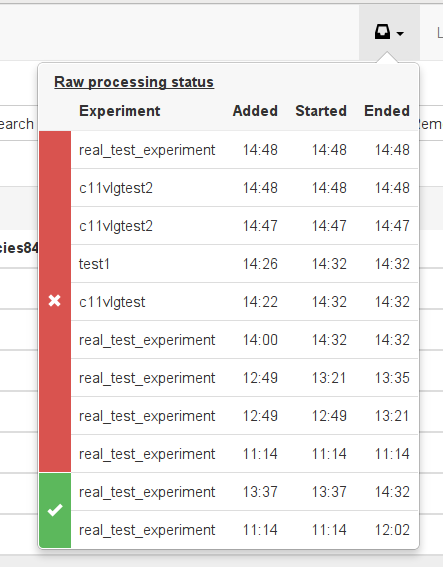
\includegraphics[width=0.4\textwidth]{web_processStatus_withData.png}
\caption{\label{fig:web_processStatus_withData}The process status dropdown.}
\end{figure}
\FloatBarrier
When pressing the inbox icon a dropdown is shown as in \refer{fig:web_processStatus_withData}displaying processing status of experiments being processed.
There are four different status a processing can have: Waiting, Running, Complete and Failed.
These are grouped together with a yellow color for waiting, blue for running, green for complete and red for failed.
\subsubsection{The process status dropdown}
\begin{figure}[h]
\centering
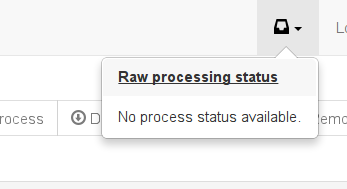
\includegraphics[width=0.5\textwidth]{web_processStatus_noData.png}
\caption{\label{fig:web_processStatus_noData}The process status dropdown with no status available.}
\end{figure}
\FloatBarrier

If there are no processes status available the user will see the text as shown in \refer{fig:web_processStatus_noData}

\subsubsection{The upload view}
%figure X7
\begin{figure}[h]
\centering
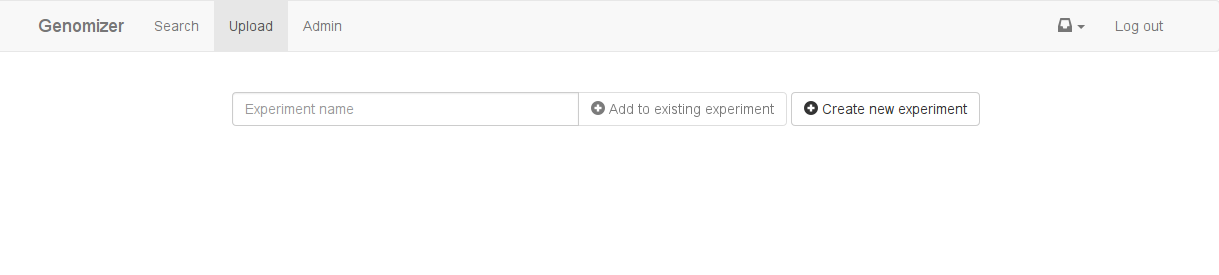
\includegraphics[width=1\textwidth]{web_upload_uploadView.png}
\caption{\label{fig:web_upload_uploadView}The upload view.}
\end{figure}

When the user clicks the upload tab in the navigation bar, the view in \refer{fig:web_upload_uploadView} will appear. The user has the option to create a new and fresh experiment or to load an existing experiment by entering its experiment name. 
%figure X8
\begin{figure}[h]
\centering
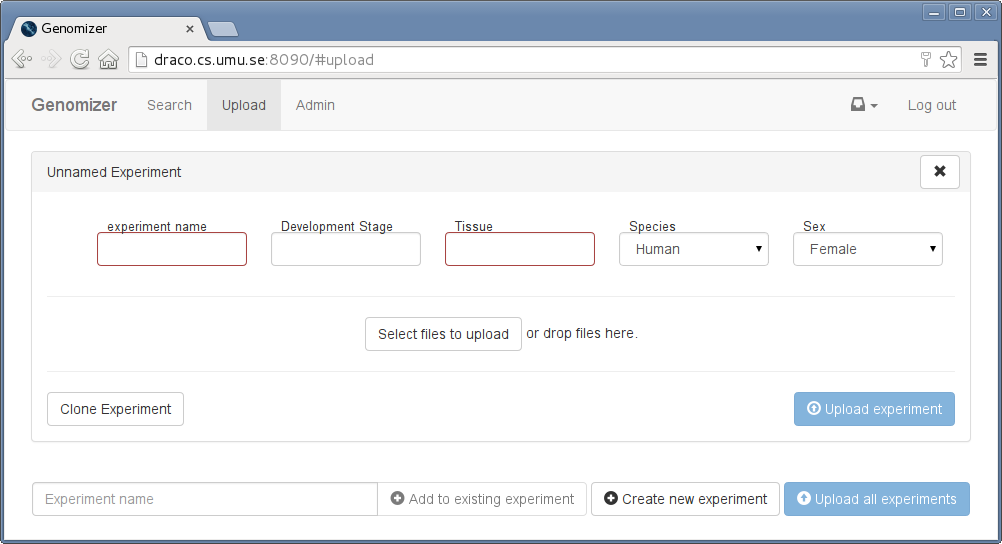
\includegraphics[width=1\textwidth]{web_upload_newExperiment.png}
\caption{\label{fig:web_upload_newExperiment}Creating a new experiment.}
\end{figure}

After clicking the “Create new experiment” button, the view in \refer{fig:web_upload_newExperiment} will appear. Here the user can input the annotations for the experiment through either freetext fields or drop-down lists. If a freetext field has a red border around it, that annotation is required and the experiment can not be uploaded before all required fields has been filled in and at least one file has been added.

The user can create more empty experiments by clicking the "Create new experiment" button and a new, empty, experiment will be placed below the first experiment.

The user can fill in annotations in one experiment that should be the same for several experiments. By clicking the "Clone experiment" button, a copy of the experiment's annotations will be appended as a new experiment. The user can change the annotations that should be different from the cloned experiment.

Up in the corner of the experiment is a button that can remove the unwanted experiment from the view. 

To add files to the experiments the user can browse for local files and upload them by clicking the “Select files to upload” button. The user will only see file types that have to do with experiments but have the ability to search for all file types. There is also a way of adding files to the experiment by dragging them from a file browser and dropping it onto the experiment "drag and drop".

An experiment can only contain two RAW-files and if the user tries to upload more a message with this information will appear and the experiment cannot be uploaded before the extra RAW-file/s is removed. 

To add files to a existing experiment the user types the name of the experiment in the field next to the "Upload to existing experiment" and clicks the button. If the experiment exists on the server it will appear in the experiment view the same way that a new experiment is shown. A existing experiments annotations cannot be changed from this view and if there is any files already in this experiment they cannot be manipulated. Adding new files to existing experiments works the same way as to a new experiment.

%figure X9
\begin{figure}[h]
\centering
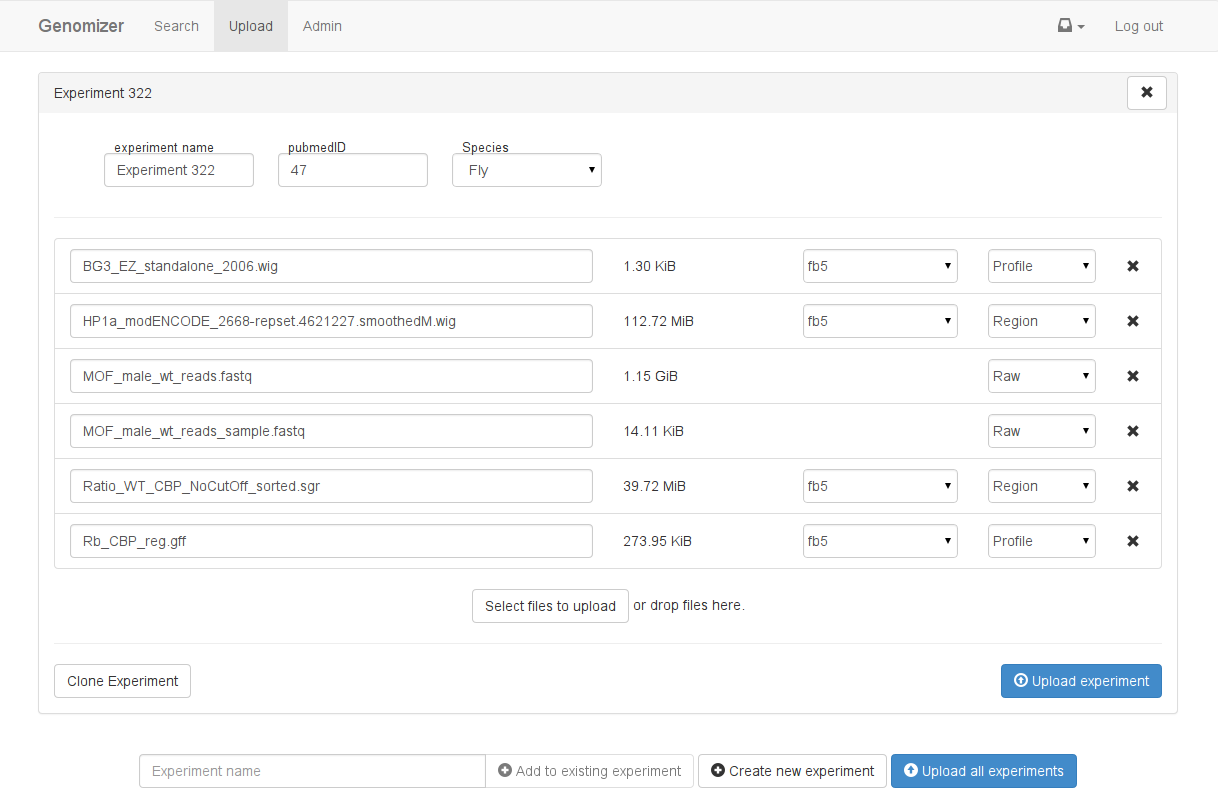
\includegraphics[width=1\textwidth]{web_upload_fileUpload.png}
\caption{\label{fig:web_upload_fileUpload}Files selected for upload.}
\end{figure}
 
When the user selects files, they will appear below the annotations as in Figure \refer{fig:web_upload_fileUpload}. The file name is displayed in a text field on the left side of the file view. Next to the file name is a box that shows the size of the selected file in a human friendly format (B, KiB, MiB, GiB, TiB). On the right side there is an option to select what type of file is being uploaded and an option to remove the file from the experiment. If the file type is either profile or region, there is an option to select what genome release the file is mapped to. The file type option will automatically be filled in with a guessed value depending on the file ending as follows: fastq files are considered raw and all other formats (sgr, wig, gff) are profile.

When the user is done selecting files, filling in annotations and clicks the “Upload experiment” button the experiment view will be minimized showing only the name of the experiment and the progressbar of the files beeing uploaded. When the progressbar is done it turns green and now the experiment with all the files has been uploaded to the server. The user also has a way of uploading several experiments at the same time by clicking "Upload all experiments".

\subsubsection{Systemadministration view}

This part of the web application is only accessible if the user have administrator-rights. It is integrated with the rest of the web UI and accessible through an admin-tab. The administrator can through this site see all existing annotations, add new annotations and edit existing ones.
The startpage of this section has a Create New Annotations button, a list of existing annotations in the database and an edit button per existing annotation. 
The view currently looks like in \refer{adm__web_annotationView}. 

\begin{figure}[h]
 \addImage{web_SysadminAnnotationView.jpg}
 \caption{The startpage for the administrator in the web client}
 \label{adm__web_annotationView}
\end{figure}

For each annotation in the annotations list, an Edit button is available. 
When pressed, it will take you to a page in which you can edit the selected annotation to change its name and what values the drop-down list will have if it's not a freetext field (See \refer{adm_web_editView}). 

\begin{figure}[h]
 \addImage{web_SysadminEditView.jpg}
 \caption{The edit annotation view}
 \label{adm_web_editView}
\end{figure}
In the edit page the admin can see the attributes of the chosen annotation and is able to delete the chosen annotation or change it's information.
The delete Annotation button will delete the whole annotation and for that reason two popup windows will appear to make sure that the administrator is sure of the action.\\
The administrator can change the list of annotation values and the site will automatically check whether 
something is added, removed or both and sends a request to change the annotation values to the server when the Update Annotation button is clicked.

If the admin clicks on Create new annotation from the admin startpage, another view will open with the following structure:
\begin{itemize}
 \item Annotation Name
 \subitem Admin can enter a name for the annotation
 
 \item Annotation Types
 \subitem Yes/No/Unknown - this will create a drop-down list with those three options.
 \subitem Freetext - will create an annotation that the users will be able to enter anything.
 \subitem Drop-down list - will enable a fourth field enabling the admin to enter which items that this list will contain.
 
 \item Forced Annotation
 \subitem Admin can choose if the new annotation should be forced for users to enter. 
\end{itemize}

A Create Annotation will, if all necessary information has been entered, result in a popup (see \refer{adm_web_createPopup}) showing the resulting annotation and if confirmed, the annotation is added to the database. 
If canceled the administrator can keep making changes or go back to exit this view. If not all values is entered the admin will be alerted of the mistake and nothing will be created.

\begin{figure}[h]
 \addImage{web_SysadminCreateAnnotationConfirm.jpg}
 \caption{The confirm annotation popup}
 \label{adm_web_createPopup}
\end{figure}

The example in \refer{adm_web_createPopup} will result in a drop-down annotation with the name ProgrammingLanguages and possible values: Java, Javascript, C++, C\# and Objective-C  with Java as default and is not forced.

A back button which takes the user back to the annotations start page is also available in this view. In \refer{adm_web_createView} the create annotation view can be seen.

\begin{figure}[t]
 \addImage{web_SysadminCreateAnnotation.jpg}
 \caption{The view for administrators where new annotations can be created}
 \label{adm_web_createView}
\end{figure}

\subsection{Setting up the application}
To setup the application, move the content of the folder called app in genomizer-web to the desired location from where the application should be run. To run the webpage open a web browser and enter the url to the folder which contains the \texttt{index.html} file(where the content of app was placed).
Ex. given that the genomizer-web folder is placed in my home folder and i want to put the webpage in a folder called public\_html which is also in my home folder. In linux i do the following steps.
\begin{enumerate}
	\item Navigate to the app folder: \texttt{“cd ~/genomizer-web/app/”}
	\item Move the contents of app to the folder called public\_html: \texttt{“mv * ~/public\_html/”}
	\item Given that the url to the pubilc\_html folder is: \filePath{“www8.cs.umu.se/~c11abc/”}
	\item To run the application start a web browser and type \filePath{“www8.cs.umu.se/~c11abc/”}
\end{enumerate}
This will open the webpage in the browser.


